\section{Graphical Transformations}
\subsection{Introduction To Graphical Transformations}
\begin{definition}[Graphical Transformations]
	A mathematical operation that alters the position, size or orientation of a function's graph on a coordinate plane, without changing its basic shape.
\end{definition}
	\subsubsection{Vertical}
		\begin{definition}[Vertical Transformation]
		\hfill
			$$f(x) + k \quad \text{Shift Up}$$
			$$f(x) - k \quad \text{Shift Down}$$
		\end{definition}
		\begin{example}[Vertical Transformation]
		\hfill
			$$f(x) = x^2 + 3$$
			\begin{center}
			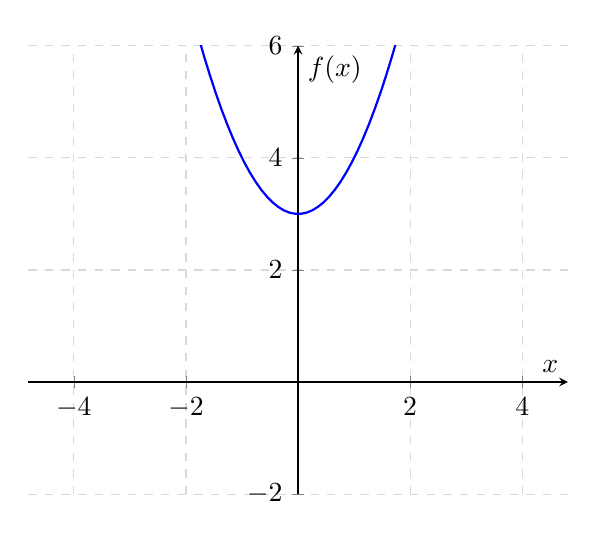
\begin{tikzpicture}
				\begin{axis}[
				    axis lines = center,
				    xlabel = $x$,
				    ylabel = $f(x)$,
				    xmin = -4, xmax = 4,
				    ymin = -2, ymax = 6,
				    grid = both,
				    grid style = {dashed, gray!30},
				    axis equal
				]
				    \addplot [domain=-5:5, samples=100, thick, blue] {x^2 + 3};
				\end{axis}
			\end{tikzpicture}
			\end{center}
			\textbf{Note: } Key points are $(1, 1) \, , (0, 0) \, , (-1, 1)$.
		\end{example}
	\subsubsection{Horizontal}
		\begin{definition}[Horizontal Transformation]
			$$f(x + h) \quad \text{Shift Left}$$
			$$f(x - h) \quad \text{Shift Right}$$
		\end{definition}
		\begin{example}[Horizontal Transformation]
			$$f(x) = |x + 2|$$
			\begin{center}
			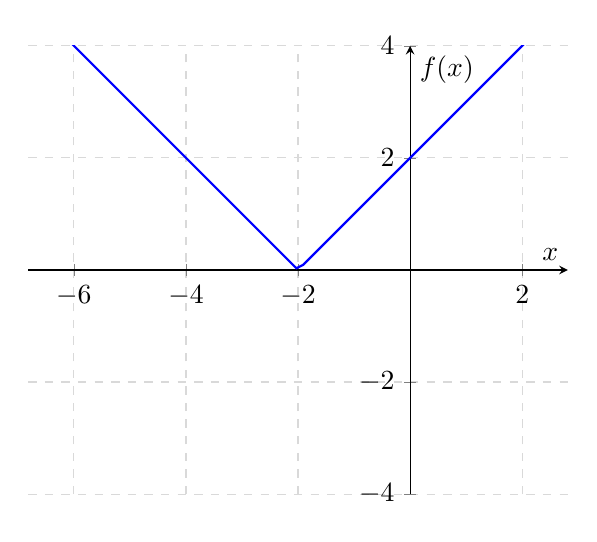
\begin{tikzpicture}
				\begin{axis}[
				    axis lines = center,
				    xlabel = $x$,
				    ylabel = $f(x)$,
				    xmin = -6, xmax = 2,
				    ymin = -4, ymax = 4,
				    grid = both,
				    grid style = {dashed, gray!30},
				    axis equal
				]
				    \addplot [domain=-7:5, samples=100, thick, blue] {abs(x + 2)};
				\end{axis}
			\end{tikzpicture}
			\end{center}
			\textbf{Note: } Key points are $(1, 1) \, , (0, 0) \, , (-1, 1)$.
		\end{example}
